\documentclass[1p]{elsarticle_modified}
%\bibliographystyle{elsarticle-num}

%\usepackage[colorlinks]{hyperref}
%\usepackage{abbrmath_seonhwa} %\Abb, \Ascr, \Acal ,\Abf, \Afrak
\usepackage{amsfonts}
\usepackage{amssymb}
\usepackage{amsmath}
\usepackage{amsthm}
\usepackage{scalefnt}
\usepackage{amsbsy}
\usepackage{kotex}
\usepackage{caption}
\usepackage{subfig}
\usepackage{color}
\usepackage{graphicx}
\usepackage{xcolor} %% white, black, red, green, blue, cyan, magenta, yellow
\usepackage{float}
\usepackage{setspace}
\usepackage{hyperref}

\usepackage{tikz}
\usetikzlibrary{arrows}

\usepackage{multirow}
\usepackage{array} % fixed length table
\usepackage{hhline}

%%%%%%%%%%%%%%%%%%%%%
\makeatletter
\renewcommand*\env@matrix[1][\arraystretch]{%
	\edef\arraystretch{#1}%
	\hskip -\arraycolsep
	\let\@ifnextchar\new@ifnextchar
	\array{*\c@MaxMatrixCols c}}
\makeatother %https://tex.stackexchange.com/questions/14071/how-can-i-increase-the-line-spacing-in-a-matrix
%%%%%%%%%%%%%%%

\usepackage[normalem]{ulem}

\newcommand{\msout}[1]{\ifmmode\text{\sout{\ensuremath{#1}}}\else\sout{#1}\fi}
%SOURCE: \msout is \stkout macro in https://tex.stackexchange.com/questions/20609/strikeout-in-math-mode

\newcommand{\cancel}[1]{
	\ifmmode
	{\color{red}\msout{#1}}
	\else
	{\color{red}\sout{#1}}
	\fi
}

\newcommand{\add}[1]{
	{\color{blue}\uwave{#1}}
}

\newcommand{\replace}[2]{
	\ifmmode
	{\color{red}\msout{#1}}{\color{blue}\uwave{#2}}
	\else
	{\color{red}\sout{#1}}{\color{blue}\uwave{#2}}
	\fi
}

\newcommand{\Sol}{\mathcal{S}} %segment
\newcommand{\D}{D} %diagram
\newcommand{\A}{\mathcal{A}} %arc


%%%%%%%%%%%%%%%%%%%%%%%%%%%%%5 test

\def\sl{\operatorname{\textup{SL}}(2,\Cbb)}
\def\psl{\operatorname{\textup{PSL}}(2,\Cbb)}
\def\quan{\mkern 1mu \triangleright \mkern 1mu}

\theoremstyle{definition}
\newtheorem{thm}{Theorem}[section]
\newtheorem{prop}[thm]{Proposition}
\newtheorem{lem}[thm]{Lemma}
\newtheorem{ques}[thm]{Question}
\newtheorem{cor}[thm]{Corollary}
\newtheorem{defn}[thm]{Definition}
\newtheorem{exam}[thm]{Example}
\newtheorem{rmk}[thm]{Remark}
\newtheorem{alg}[thm]{Algorithm}

\newcommand{\I}{\sqrt{-1}}
\begin{document}

%\begin{frontmatter}
%
%\title{Boundary parabolic representations of knots up to 8 crossings}
%
%%% Group authors per affiliation:
%\author{Yunhi Cho} 
%\address{Department of Mathematics, University of Seoul, Seoul, Korea}
%\ead{yhcho@uos.ac.kr}
%
%
%\author{Seonhwa Kim} %\fnref{s_kim}}
%\address{Center for Geometry and Physics, Institute for Basic Science, Pohang, 37673, Korea}
%\ead{ryeona17@ibs.re.kr}
%
%\author{Hyuk Kim}
%\address{Department of Mathematical Sciences, Seoul National University, Seoul 08826, Korea}
%\ead{hyukkim@snu.ac.kr}
%
%\author{Seokbeom Yoon}
%\address{Department of Mathematical Sciences, Seoul National University, Seoul, 08826,  Korea}
%\ead{sbyoon15@snu.ac.kr}
%
%\begin{abstract}
%We find all boundary parabolic representation of knots up to 8 crossings.
%
%\end{abstract}
%\begin{keyword}
%    \MSC[2010] 57M25 
%\end{keyword}
%
%\end{frontmatter}

%\linenumbers
%\tableofcontents
%
\newcommand\colored[1]{\textcolor{white}{\rule[-0.35ex]{0.8em}{1.4ex}}\kern-0.8em\color{red} #1}%
%\newcommand\colored[1]{\textcolor{white}{ #1}\kern-2.17ex	\textcolor{white}{ #1}\kern-1.81ex	\textcolor{white}{ #1}\kern-2.15ex\color{red}#1	}

{\Large $\underline{11n_{170}~(K11n_{170})}$}

\setlength{\tabcolsep}{10pt}
\renewcommand{\arraystretch}{1.6}
\vspace{1cm}\begin{tabular}{m{100pt}>{\centering\arraybackslash}m{274pt}}
\multirow{5}{120pt}{
	\centering
	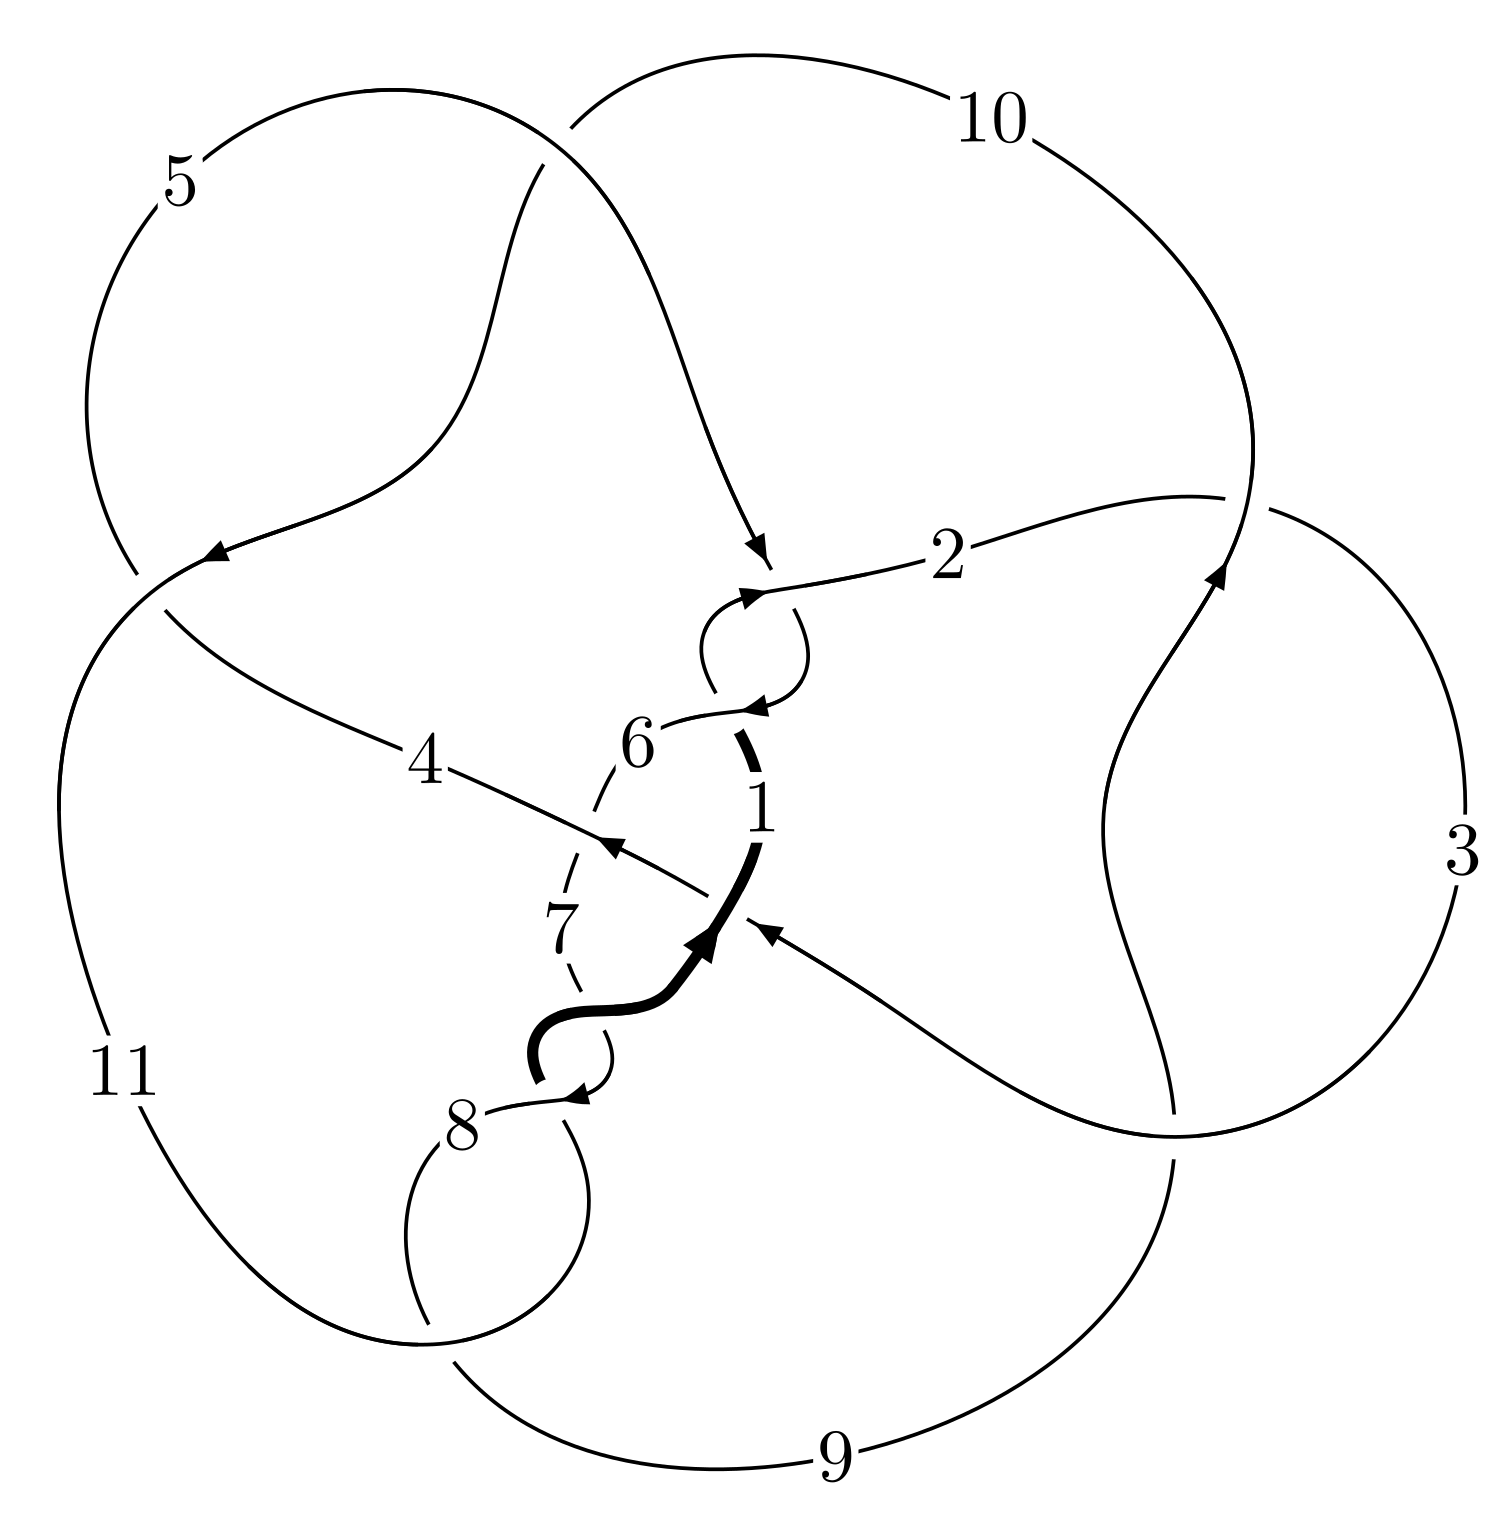
\includegraphics[width=112pt]{../../../GIT/diagram.site/Diagrams/png/786_11n_170.png}\\
\ \ \ A knot diagram\footnotemark}&
\allowdisplaybreaks
\textbf{Linearized knot diagam} \\
\cline{2-2}
 &
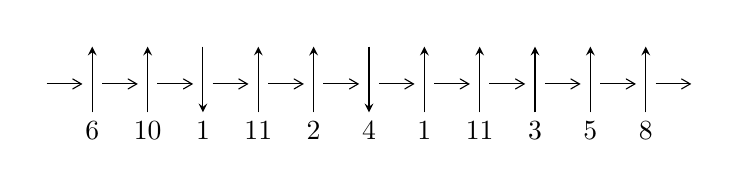
\begin{tikzpicture}[x=20pt, y=17pt]
	% nodes
	\node (C0) at (0, 0) {};
	\node (C1) at (1, 0) {};
	\node (C1U) at (1, +1) {};
	\node (C1D) at (1, -1) {6};

	\node (C2) at (2, 0) {};
	\node (C2U) at (2, +1) {};
	\node (C2D) at (2, -1) {10};

	\node (C3) at (3, 0) {};
	\node (C3U) at (3, +1) {};
	\node (C3D) at (3, -1) {1};

	\node (C4) at (4, 0) {};
	\node (C4U) at (4, +1) {};
	\node (C4D) at (4, -1) {11};

	\node (C5) at (5, 0) {};
	\node (C5U) at (5, +1) {};
	\node (C5D) at (5, -1) {2};

	\node (C6) at (6, 0) {};
	\node (C6U) at (6, +1) {};
	\node (C6D) at (6, -1) {4};

	\node (C7) at (7, 0) {};
	\node (C7U) at (7, +1) {};
	\node (C7D) at (7, -1) {1};

	\node (C8) at (8, 0) {};
	\node (C8U) at (8, +1) {};
	\node (C8D) at (8, -1) {11};

	\node (C9) at (9, 0) {};
	\node (C9U) at (9, +1) {};
	\node (C9D) at (9, -1) {3};

	\node (C10) at (10, 0) {};
	\node (C10U) at (10, +1) {};
	\node (C10D) at (10, -1) {5};

	\node (C11) at (11, 0) {};
	\node (C11U) at (11, +1) {};
	\node (C11D) at (11, -1) {8};
	\node (C12) at (12, 0) {};

	% arrows
	\draw[->,>={angle 60}]
	(C0) edge (C1) (C1) edge (C2) (C2) edge (C3) (C3) edge (C4) (C4) edge (C5) (C5) edge (C6) (C6) edge (C7) (C7) edge (C8) (C8) edge (C9) (C9) edge (C10) (C10) edge (C11) (C11) edge (C12) ;	\draw[->,>=stealth]
	(C1D) edge (C1U) (C2D) edge (C2U) (C3U) edge (C3D) (C4D) edge (C4U) (C5D) edge (C5U) (C6U) edge (C6D) (C7D) edge (C7U) (C8D) edge (C8U) (C9D) edge (C9U) (C10D) edge (C10U) (C11D) edge (C11U) ;
	\end{tikzpicture} \\
\hhline{~~} \\& 
\textbf{Solving Sequence} \\ \cline{2-2} 
 &
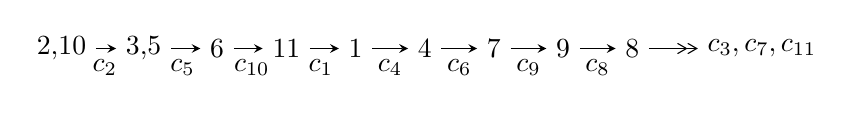
\begin{tikzpicture}[x=25pt, y=7pt]
	% node
	\node (A0) at (-1/8, 0) {2,10};
	\node (A1) at (17/16, 0) {3,5};
	\node (A2) at (17/8, 0) {6};
	\node (A3) at (25/8, 0) {11};
	\node (A4) at (33/8, 0) {1};
	\node (A5) at (41/8, 0) {4};
	\node (A6) at (49/8, 0) {7};
	\node (A7) at (57/8, 0) {9};
	\node (A8) at (65/8, 0) {8};
	\node (C1) at (1/2, -1) {$c_{2}$};
	\node (C2) at (13/8, -1) {$c_{5}$};
	\node (C3) at (21/8, -1) {$c_{10}$};
	\node (C4) at (29/8, -1) {$c_{1}$};
	\node (C5) at (37/8, -1) {$c_{4}$};
	\node (C6) at (45/8, -1) {$c_{6}$};
	\node (C7) at (53/8, -1) {$c_{9}$};
	\node (C8) at (61/8, -1) {$c_{8}$};
	\node (A9) at (10, 0) {$c_{3},c_{7},c_{11}$};

	% edge
	\draw[->,>=stealth]	
	(A0) edge (A1) (A1) edge (A2) (A2) edge (A3) (A3) edge (A4) (A4) edge (A5) (A5) edge (A6) (A6) edge (A7) (A7) edge (A8) ;
	\draw[->>,>={angle 60}]	
	(A8) edge (A9);
\end{tikzpicture} \\ 

\end{tabular} \\

\footnotetext{
The image of knot diagram is generated by the software ``\textbf{Draw programme}" developed by Andrew Bartholomew(\url{http://www.layer8.co.uk/maths/draw/index.htm\#Running-draw}), where we modified some parts for our purpose(\url{https://github.com/CATsTAILs/LinksPainter}).
}\phantom \\ \newline 
\centering \textbf{Ideals for irreducible components\footnotemark of $X_{\text{par}}$} 
 
\begin{align*}
I^u_{1}&=\langle 
-25 u^{16}-25 u^{15}+\cdots+18 b+137,\;a-1,\;u^{17}+6 u^{15}+\cdots- u-1\rangle \\
I^u_{2}&=\langle 
-5.20249\times10^{17} u^{23}+5.01695\times10^{18} u^{22}+\cdots+1.95146\times10^{19} b+5.92561\times10^{20},\\
\phantom{I^u_{2}}&\phantom{= \langle  }-1.39688\times10^{24} u^{23}+6.26259\times10^{24} u^{22}+\cdots+1.95641\times10^{25} a+5.44584\times10^{26},\\
\phantom{I^u_{2}}&\phantom{= \langle  }u^{24}- u^{23}+\cdots+224 u+173\rangle \\
I^u_{3}&=\langle 
u^9- u^8+5 u^7-3 u^6+12 u^5-2 u^4+10 u^3+u^2+3 b+u-2,\;a+1,\\
\phantom{I^u_{3}}&\phantom{= \langle  }u^{10}+4 u^8- u^7+6 u^6-2 u^5+2 u^4- u^3- u^2- u+1\rangle \\
\\
\end{align*}
\raggedright * 3 irreducible components of $\dim_{\mathbb{C}}=0$, with total 51 representations.\\
\footnotetext{All coefficients of polynomials are rational numbers. But the coefficients are sometimes approximated in decimal forms when there is not enough margin.}
\newpage
\renewcommand{\arraystretch}{1}
\centering \section*{I. $I^u_{1}= \langle -25 u^{16}-25 u^{15}+\cdots+18 b+137,\;a-1,\;u^{17}+6 u^{15}+\cdots- u-1 \rangle$}
\flushleft \textbf{(i) Arc colorings}\\
\begin{tabular}{m{7pt} m{180pt} m{7pt} m{180pt} }
\flushright $a_{2}=$&$\begin{pmatrix}1\\0\end{pmatrix}$ \\
\flushright $a_{10}=$&$\begin{pmatrix}0\\u\end{pmatrix}$ \\
\flushright $a_{3}=$&$\begin{pmatrix}1\\- u^2\end{pmatrix}$ \\
\flushright $a_{5}=$&$\begin{pmatrix}1\\1.38889 u^{16}+1.38889 u^{15}+\cdots+4.77778 u-7.61111\end{pmatrix}$ \\
\flushright $a_{6}=$&$\begin{pmatrix}1.38889 u^{16}+1.38889 u^{15}+\cdots+4.77778 u-6.61111\\1.38889 u^{16}+1.38889 u^{15}+\cdots+4.77778 u-7.61111\end{pmatrix}$ \\
\flushright $a_{11}=$&$\begin{pmatrix}u\\1.38889 u^{16}-1.61111 u^{15}+\cdots-5.22222 u+1.38889\end{pmatrix}$ \\
\flushright $a_{1}=$&$\begin{pmatrix}-0.277778 u^{16}+1.05556 u^{15}+\cdots+3.44444 u-2.61111\\-\frac{5}{3} u^{16}-\frac{1}{3} u^{15}+\cdots-\frac{4}{3} u+4\end{pmatrix}$ \\
\flushright $a_{4}=$&$\begin{pmatrix}u^2+1\\-\frac{2}{9} u^{16}+\frac{25}{9} u^{15}+\cdots+\frac{68}{9} u-\frac{56}{9}\end{pmatrix}$ \\
\flushright $a_{7}=$&$\begin{pmatrix}\frac{1}{6} u^{16}+\frac{1}{2} u^{15}+\cdots+\frac{7}{3} u-\frac{7}{6}\\\frac{55}{9} u^{16}-\frac{23}{9} u^{15}+\cdots-\frac{43}{9} u-\frac{83}{9}\end{pmatrix}$ \\
\flushright $a_{9}=$&$\begin{pmatrix}- u\\u^3+u\end{pmatrix}$ \\
\flushright $a_{8}=$&$\begin{pmatrix}-1.38889 u^{16}+0.611111 u^{15}+\cdots-0.777778 u+1.61111\\-\frac{26}{9} u^{16}+\frac{7}{9} u^{15}+\cdots+\frac{2}{9} u+\frac{40}{9}\end{pmatrix}$\\ \flushright $a_{8}=$&$\begin{pmatrix}-1.38889 u^{16}+0.611111 u^{15}+\cdots-0.777778 u+1.61111\\-\frac{26}{9} u^{16}+\frac{7}{9} u^{15}+\cdots+\frac{2}{9} u+\frac{40}{9}\end{pmatrix}$\\&\end{tabular}
\flushleft \textbf{(ii) Obstruction class $= -1$}\\~\\
\flushleft \textbf{(iii) Cusp Shapes $= \frac{103}{9} u^{16}-\frac{2}{9} u^{15}+\frac{601}{9} u^{14}+\frac{122}{9} u^{13}+\frac{1927}{9} u^{12}+\frac{542}{9} u^{11}+\frac{3436}{9} u^{10}+\frac{1481}{9} u^9+\frac{3799}{9} u^8+\frac{2359}{9} u^7+\frac{2344}{9} u^6+257 u^5+88 u^4+\frac{862}{9} u^3+\frac{40}{3} u^2+\frac{35}{9} u-\frac{170}{9}$}\\~\\
\newpage\renewcommand{\arraystretch}{1}
\flushleft \textbf{(iv) u-Polynomials at the component}\newline \\
\begin{tabular}{m{50pt}|m{274pt}}
Crossings & \hspace{64pt}u-Polynomials at each crossing \\
\hline $$\begin{aligned}c_{1},c_{5}\end{aligned}$$&$\begin{aligned}
&u^{17}-9 u^{16}+\cdots+144 u-16
\end{aligned}$\\
\hline $$\begin{aligned}c_{2},c_{4},c_{9}\\c_{10}\end{aligned}$$&$\begin{aligned}
&u^{17}+6 u^{15}+\cdots- u-1
\end{aligned}$\\
\hline $$\begin{aligned}c_{3},c_{6}\end{aligned}$$&$\begin{aligned}
&u^{17}+9 u^{15}+\cdots+3 u^2-1
\end{aligned}$\\
\hline $$\begin{aligned}c_{7},c_{8},c_{11}\end{aligned}$$&$\begin{aligned}
&u^{17}+9 u^{16}+\cdots-32 u-8
\end{aligned}$\\
\hline
\end{tabular}\\~\\
\newpage\renewcommand{\arraystretch}{1}
\flushleft \textbf{(v) Riley Polynomials at the component}\newline \\
\begin{tabular}{m{50pt}|m{274pt}}
Crossings & \hspace{64pt}Riley Polynomials at each crossing \\
\hline $$\begin{aligned}c_{1},c_{5}\end{aligned}$$&$\begin{aligned}
&y^{17}+15 y^{16}+\cdots+1408 y-256
\end{aligned}$\\
\hline $$\begin{aligned}c_{2},c_{4},c_{9}\\c_{10}\end{aligned}$$&$\begin{aligned}
&y^{17}+12 y^{16}+\cdots- y-1
\end{aligned}$\\
\hline $$\begin{aligned}c_{3},c_{6}\end{aligned}$$&$\begin{aligned}
&y^{17}+18 y^{16}+\cdots+6 y-1
\end{aligned}$\\
\hline $$\begin{aligned}c_{7},c_{8},c_{11}\end{aligned}$$&$\begin{aligned}
&y^{17}+9 y^{16}+\cdots+160 y-64
\end{aligned}$\\
\hline
\end{tabular}\\~\\
\newpage\flushleft \textbf{(vi) Complex Volumes and Cusp Shapes}
$$\begin{array}{c|c|c}  
\text{Solutions to }I^u_{1}& \I (\text{vol} + \sqrt{-1}CS) & \text{Cusp shape}\\
 \hline 
\begin{aligned}
u &= \phantom{-}0.145212 + 0.987929 I \\
a &= \phantom{-}1.00000\phantom{ +0.000000I} \\
b &= -0.861098 + 1.080220 I\end{aligned}
 & -1.58511 + 1.52682 I & \phantom{-}1.71933 - 1.54413 I \\ \hline\begin{aligned}
u &= \phantom{-}0.145212 - 0.987929 I \\
a &= \phantom{-}1.00000\phantom{ +0.000000I} \\
b &= -0.861098 - 1.080220 I\end{aligned}
 & -1.58511 - 1.52682 I & \phantom{-}1.71933 + 1.54413 I \\ \hline\begin{aligned}
u &= \phantom{-}0.594895 + 0.853325 I \\
a &= \phantom{-}1.00000\phantom{ +0.000000I} \\
b &= -0.888119 - 0.392484 I\end{aligned}
 & \phantom{-}2.52996 + 1.99554 I & \phantom{-}7.48406 - 3.24951 I \\ \hline\begin{aligned}
u &= \phantom{-}0.594895 - 0.853325 I \\
a &= \phantom{-}1.00000\phantom{ +0.000000I} \\
b &= -0.888119 + 0.392484 I\end{aligned}
 & \phantom{-}2.52996 - 1.99554 I & \phantom{-}7.48406 + 3.24951 I \\ \hline\begin{aligned}
u &= \phantom{-}0.455681 + 1.021510 I \\
a &= \phantom{-}1.00000\phantom{ +0.000000I} \\
b &= -0.09174 - 1.74935 I\end{aligned}
 & -12.10840 + 1.93472 I & \phantom{-}7.26417 - 4.67402 I \\ \hline\begin{aligned}
u &= \phantom{-}0.455681 - 1.021510 I \\
a &= \phantom{-}1.00000\phantom{ +0.000000I} \\
b &= -0.09174 + 1.74935 I\end{aligned}
 & -12.10840 - 1.93472 I & \phantom{-}7.26417 + 4.67402 I \\ \hline\begin{aligned}
u &= -0.504262 + 1.174830 I \\
a &= \phantom{-}1.00000\phantom{ +0.000000I} \\
b &= -1.088960 + 0.356976 I\end{aligned}
 & \phantom{-}0.48540 - 8.16941 I & \phantom{-}4.20960 + 6.58024 I \\ \hline\begin{aligned}
u &= -0.504262 - 1.174830 I \\
a &= \phantom{-}1.00000\phantom{ +0.000000I} \\
b &= -1.088960 - 0.356976 I\end{aligned}
 & \phantom{-}0.48540 + 8.16941 I & \phantom{-}4.20960 - 6.58024 I \\ \hline\begin{aligned}
u &= -0.449425 + 0.466610 I \\
a &= \phantom{-}1.00000\phantom{ +0.000000I} \\
b &= -0.570876 - 1.008450 I\end{aligned}
 & \phantom{-}0.75353 + 3.18135 I & \phantom{-}3.49254 + 0.13841 I \\ \hline\begin{aligned}
u &= -0.449425 - 0.466610 I \\
a &= \phantom{-}1.00000\phantom{ +0.000000I} \\
b &= -0.570876 + 1.008450 I\end{aligned}
 & \phantom{-}0.75353 - 3.18135 I & \phantom{-}3.49254 - 0.13841 I\\
 \hline 
 \end{array}$$\newpage$$\begin{array}{c|c|c}  
\text{Solutions to }I^u_{1}& \I (\text{vol} + \sqrt{-1}CS) & \text{Cusp shape}\\
 \hline 
\begin{aligned}
u &= -0.455902 + 0.433518 I \\
a &= \phantom{-}1.00000\phantom{ +0.000000I} \\
b &= -0.039420 + 0.886123 I\end{aligned}
 & -1.82684 - 1.47458 I & \phantom{-}1.47955 + 5.16393 I \\ \hline\begin{aligned}
u &= -0.455902 - 0.433518 I \\
a &= \phantom{-}1.00000\phantom{ +0.000000I} \\
b &= -0.039420 - 0.886123 I\end{aligned}
 & -1.82684 + 1.47458 I & \phantom{-}1.47955 - 5.16393 I \\ \hline\begin{aligned}
u &= -0.71525 + 1.27905 I \\
a &= \phantom{-}1.00000\phantom{ +0.000000I} \\
b &= -0.35508 + 1.52708 I\end{aligned}
 & -3.71302 - 6.55902 I & \phantom{-}3.96621 + 4.14123 I \\ \hline\begin{aligned}
u &= -0.71525 - 1.27905 I \\
a &= \phantom{-}1.00000\phantom{ +0.000000I} \\
b &= -0.35508 - 1.52708 I\end{aligned}
 & -3.71302 + 6.55902 I & \phantom{-}3.96621 - 4.14123 I \\ \hline\begin{aligned}
u &= \phantom{-}0.478551\phantom{ +0.000000I} \\
a &= \phantom{-}1.00000\phantom{ +0.000000I} \\
b &= -0.344169\phantom{ +0.000000I}\end{aligned}
 & \phantom{-}0.721984\phantom{ +0.000000I} & \phantom{-}13.8930\phantom{ +0.000000I} \\ \hline\begin{aligned}
u &= \phantom{-}0.68977 + 1.47618 I \\
a &= \phantom{-}1.00000\phantom{ +0.000000I} \\
b &= -0.43262 - 1.51053 I\end{aligned}
 & -5.4582 + 13.6098 I & \phantom{-}1.93808 - 7.30834 I \\ \hline\begin{aligned}
u &= \phantom{-}0.68977 - 1.47618 I \\
a &= \phantom{-}1.00000\phantom{ +0.000000I} \\
b &= -0.43262 + 1.51053 I\end{aligned}
 & -5.4582 - 13.6098 I & \phantom{-}1.93808 + 7.30834 I\\
 \hline 
 \end{array}$$\newpage\newpage\renewcommand{\arraystretch}{1}
\centering \section*{II. $I^u_{2}= \langle -5.20\times10^{17} u^{23}+5.02\times10^{18} u^{22}+\cdots+1.95\times10^{19} b+5.93\times10^{20},\;-1.40\times10^{24} u^{23}+6.26\times10^{24} u^{22}+\cdots+1.96\times10^{25} a+5.45\times10^{26},\;u^{24}- u^{23}+\cdots+224 u+173 \rangle$}
\flushleft \textbf{(i) Arc colorings}\\
\begin{tabular}{m{7pt} m{180pt} m{7pt} m{180pt} }
\flushright $a_{2}=$&$\begin{pmatrix}1\\0\end{pmatrix}$ \\
\flushright $a_{10}=$&$\begin{pmatrix}0\\u\end{pmatrix}$ \\
\flushright $a_{3}=$&$\begin{pmatrix}1\\- u^2\end{pmatrix}$ \\
\flushright $a_{5}=$&$\begin{pmatrix}0.0714002 u^{23}-0.320106 u^{22}+\cdots-15.5190 u-27.8359\\0.0266595 u^{23}-0.257087 u^{22}+\cdots-18.6780 u-30.3650\end{pmatrix}$ \\
\flushright $a_{6}=$&$\begin{pmatrix}0.0980596 u^{23}-0.577193 u^{22}+\cdots-34.1970 u-58.2008\\0.0266595 u^{23}-0.257087 u^{22}+\cdots-18.6780 u-30.3650\end{pmatrix}$ \\
\flushright $a_{11}=$&$\begin{pmatrix}0.470356 u^{23}-0.621434 u^{22}+\cdots+81.7674 u+16.2383\\0.329501 u^{23}-0.686697 u^{22}+\cdots+33.8837 u-21.2874\end{pmatrix}$ \\
\flushright $a_{1}=$&$\begin{pmatrix}0.450732 u^{23}-0.314505 u^{22}+\cdots+120.111 u+62.4009\\0.327683 u^{23}-0.520957 u^{22}+\cdots+55.3338 u+0.954331\end{pmatrix}$ \\
\flushright $a_{4}=$&$\begin{pmatrix}0.0595221 u^{23}+0.166006 u^{22}+\cdots+28.1599 u+41.7764\\0.497954 u^{23}-0.518732 u^{22}+\cdots+103.014 u+48.4483\end{pmatrix}$ \\
\flushright $a_{7}=$&$\begin{pmatrix}-0.645948 u^{23}+1.30849 u^{22}+\cdots-66.6364 u+32.6828\\0.142189 u^{23}+0.502228 u^{22}+\cdots+106.073 u+111.052\end{pmatrix}$ \\
\flushright $a_{9}=$&$\begin{pmatrix}- u\\u^3+u\end{pmatrix}$ \\
\flushright $a_{8}=$&$\begin{pmatrix}0.383897 u^{23}-0.657761 u^{22}+\cdots+57.2698 u+0.530339\\-0.0745968 u^{23}-0.255739 u^{22}+\cdots-52.0295 u-57.0282\end{pmatrix}$\\ \flushright $a_{8}=$&$\begin{pmatrix}0.383897 u^{23}-0.657761 u^{22}+\cdots+57.2698 u+0.530339\\-0.0745968 u^{23}-0.255739 u^{22}+\cdots-52.0295 u-57.0282\end{pmatrix}$\\&\end{tabular}
\flushleft \textbf{(ii) Obstruction class $= -1$}\\~\\
\flushleft \textbf{(iii) Cusp Shapes $= \frac{57116119689452910512704}{113087261740869136389035} u^{23}-\frac{196123354323563952367144}{113087261740869136389035} u^{22}+\cdots-\frac{343977527111163574580764}{22617452348173827277807} u-\frac{16520278039745704687355386}{113087261740869136389035}$}\\~\\
\newpage\renewcommand{\arraystretch}{1}
\flushleft \textbf{(iv) u-Polynomials at the component}\newline \\
\begin{tabular}{m{50pt}|m{274pt}}
Crossings & \hspace{64pt}u-Polynomials at each crossing \\
\hline $$\begin{aligned}c_{1},c_{5}\end{aligned}$$&$\begin{aligned}
&(u^3+u^2+2 u+1)^8
\end{aligned}$\\
\hline $$\begin{aligned}c_{2},c_{4},c_{9}\\c_{10}\end{aligned}$$&$\begin{aligned}
&u^{24}- u^{23}+\cdots+224 u+173
\end{aligned}$\\
\hline $$\begin{aligned}c_{3},c_{6}\end{aligned}$$&$\begin{aligned}
&u^{24}-3 u^{23}+\cdots-14 u+19
\end{aligned}$\\
\hline $$\begin{aligned}c_{7},c_{8},c_{11}\end{aligned}$$&$\begin{aligned}
&(u^4- u^3+u^2+1)^6
\end{aligned}$\\
\hline
\end{tabular}\\~\\
\newpage\renewcommand{\arraystretch}{1}
\flushleft \textbf{(v) Riley Polynomials at the component}\newline \\
\begin{tabular}{m{50pt}|m{274pt}}
Crossings & \hspace{64pt}Riley Polynomials at each crossing \\
\hline $$\begin{aligned}c_{1},c_{5}\end{aligned}$$&$\begin{aligned}
&(y^3+3 y^2+2 y-1)^8
\end{aligned}$\\
\hline $$\begin{aligned}c_{2},c_{4},c_{9}\\c_{10}\end{aligned}$$&$\begin{aligned}
&y^{24}+15 y^{23}+\cdots+196176 y+29929
\end{aligned}$\\
\hline $$\begin{aligned}c_{3},c_{6}\end{aligned}$$&$\begin{aligned}
&y^{24}+7 y^{23}+\cdots+11812 y+361
\end{aligned}$\\
\hline $$\begin{aligned}c_{7},c_{8},c_{11}\end{aligned}$$&$\begin{aligned}
&(y^4+y^3+3 y^2+2 y+1)^6
\end{aligned}$\\
\hline
\end{tabular}\\~\\
\newpage\flushleft \textbf{(vi) Complex Volumes and Cusp Shapes}
$$\begin{array}{c|c|c}  
\text{Solutions to }I^u_{2}& \I (\text{vol} + \sqrt{-1}CS) & \text{Cusp shape}\\
 \hline 
\begin{aligned}
u &= -0.296109 + 0.977179 I \\
a &= -1.273900 + 0.388233 I \\
b &= \phantom{-}0.569840\phantom{ +0.000000I}\end{aligned}
 & -4.03235 - 1.41510 I & \phantom{-}5.19277 + 4.90874 I \\ \hline\begin{aligned}
u &= -0.296109 - 0.977179 I \\
a &= -1.273900 - 0.388233 I \\
b &= \phantom{-}0.569840\phantom{ +0.000000I}\end{aligned}
 & -4.03235 + 1.41510 I & \phantom{-}5.19277 - 4.90874 I \\ \hline\begin{aligned}
u &= -0.850110 + 0.413706 I \\
a &= -0.382281 - 1.077960 I \\
b &= \phantom{-}0.569840\phantom{ +0.000000I}\end{aligned}
 & \phantom{-}2.96939 + 3.16396 I & \phantom{-}8.84625 - 2.56480 I \\ \hline\begin{aligned}
u &= -0.850110 - 0.413706 I \\
a &= -0.382281 + 1.077960 I \\
b &= \phantom{-}0.569840\phantom{ +0.000000I}\end{aligned}
 & \phantom{-}2.96939 - 3.16396 I & \phantom{-}8.84625 + 2.56480 I \\ \hline\begin{aligned}
u &= -0.338066 + 1.017770 I \\
a &= -1.64492 + 0.24451 I \\
b &= \phantom{-}0.215080 - 1.307140 I\end{aligned}
 & -8.16994 - 1.41302 I & -1.33649 - 1.92930 I \\ \hline\begin{aligned}
u &= -0.338066 - 1.017770 I \\
a &= -1.64492 - 0.24451 I \\
b &= \phantom{-}0.215080 + 1.307140 I\end{aligned}
 & -8.16994 + 1.41302 I & -1.33649 + 1.92930 I \\ \hline\begin{aligned}
u &= \phantom{-}0.770941 + 0.758235 I \\
a &= -0.292232 + 0.824041 I \\
b &= \phantom{-}0.569840\phantom{ +0.000000I}\end{aligned}
 & \phantom{-}2.96939 + 3.16396 I & \phantom{-}8.84625 - 2.56480 I \\ \hline\begin{aligned}
u &= \phantom{-}0.770941 - 0.758235 I \\
a &= -0.292232 - 0.824041 I \\
b &= \phantom{-}0.569840\phantom{ +0.000000I}\end{aligned}
 & \phantom{-}2.96939 - 3.16396 I & \phantom{-}8.84625 + 2.56480 I \\ \hline\begin{aligned}
u &= \phantom{-}0.105985 + 0.888600 I \\
a &= \phantom{-}0.45731 + 1.37162 I \\
b &= \phantom{-}0.215080 + 1.307140 I\end{aligned}
 & -1.168190 - 0.335841 I & \phantom{-}2.31698 - 0.41465 I \\ \hline\begin{aligned}
u &= \phantom{-}0.105985 - 0.888600 I \\
a &= \phantom{-}0.45731 - 1.37162 I \\
b &= \phantom{-}0.215080 - 1.307140 I\end{aligned}
 & -1.168190 + 0.335841 I & \phantom{-}2.31698 + 0.41465 I\\
 \hline 
 \end{array}$$\newpage$$\begin{array}{c|c|c}  
\text{Solutions to }I^u_{2}& \I (\text{vol} + \sqrt{-1}CS) & \text{Cusp shape}\\
 \hline 
\begin{aligned}
u &= -0.273584 + 1.104980 I \\
a &= -0.168598 - 1.335650 I \\
b &= \phantom{-}0.215080 - 1.307140 I\end{aligned}
 & -1.16819 - 5.99209 I & \phantom{-}2.31698 + 5.54425 I \\ \hline\begin{aligned}
u &= -0.273584 - 1.104980 I \\
a &= -0.168598 + 1.335650 I \\
b &= \phantom{-}0.215080 + 1.307140 I\end{aligned}
 & -1.16819 + 5.99209 I & \phantom{-}2.31698 - 5.54425 I \\ \hline\begin{aligned}
u &= -1.170350 + 0.551735 I \\
a &= \phantom{-}0.218758 - 0.656129 I \\
b &= \phantom{-}0.215080 + 1.307140 I\end{aligned}
 & -1.168190 - 0.335841 I & \phantom{-}2.31698 - 0.41465 I \\ \hline\begin{aligned}
u &= -1.170350 - 0.551735 I \\
a &= \phantom{-}0.218758 + 0.656129 I \\
b &= \phantom{-}0.215080 - 1.307140 I\end{aligned}
 & -1.168190 + 0.335841 I & \phantom{-}2.31698 + 0.41465 I \\ \hline\begin{aligned}
u &= -0.002161 + 1.359780 I \\
a &= -0.718280 + 0.218903 I \\
b &= \phantom{-}0.569840\phantom{ +0.000000I}\end{aligned}
 & -4.03235 + 1.41510 I & \phantom{-}5.19277 - 4.90874 I \\ \hline\begin{aligned}
u &= -0.002161 - 1.359780 I \\
a &= -0.718280 - 0.218903 I \\
b &= \phantom{-}0.569840\phantom{ +0.000000I}\end{aligned}
 & -4.03235 - 1.41510 I & \phantom{-}5.19277 + 4.90874 I \\ \hline\begin{aligned}
u &= -0.23515 + 1.45919 I \\
a &= -0.977489 - 0.499948 I \\
b &= \phantom{-}0.215080 - 1.307140 I\end{aligned}
 & -8.16994 - 4.24323 I & -1.33649 + 7.88819 I \\ \hline\begin{aligned}
u &= -0.23515 - 1.45919 I \\
a &= -0.977489 + 0.499948 I \\
b &= \phantom{-}0.215080 + 1.307140 I\end{aligned}
 & -8.16994 + 4.24323 I & -1.33649 - 7.88819 I \\ \hline\begin{aligned}
u &= \phantom{-}1.52200 + 0.17911 I \\
a &= -0.093025 + 0.736956 I \\
b &= \phantom{-}0.215080 - 1.307140 I\end{aligned}
 & -1.16819 - 5.99209 I & \phantom{-}2.31698 + 5.54425 I \\ \hline\begin{aligned}
u &= \phantom{-}1.52200 - 0.17911 I \\
a &= -0.093025 - 0.736956 I \\
b &= \phantom{-}0.215080 + 1.307140 I\end{aligned}
 & -1.16819 + 5.99209 I & \phantom{-}2.31698 - 5.54425 I\\
 \hline 
 \end{array}$$\newpage$$\begin{array}{c|c|c}  
\text{Solutions to }I^u_{2}& \I (\text{vol} + \sqrt{-1}CS) & \text{Cusp shape}\\
 \hline 
\begin{aligned}
u &= \phantom{-}0.95938 + 1.30878 I \\
a &= -0.810903 - 0.414746 I \\
b &= \phantom{-}0.215080 + 1.307140 I\end{aligned}
 & -8.16994 + 4.24323 I & -1.33649 - 7.88819 I \\ \hline\begin{aligned}
u &= \phantom{-}0.95938 - 1.30878 I \\
a &= -0.810903 + 0.414746 I \\
b &= \phantom{-}0.215080 - 1.307140 I\end{aligned}
 & -8.16994 - 4.24323 I & -1.33649 + 7.88819 I \\ \hline\begin{aligned}
u &= \phantom{-}0.30723 + 1.75680 I \\
a &= -0.594791 + 0.088414 I \\
b &= \phantom{-}0.215080 + 1.307140 I\end{aligned}
 & -8.16994 + 1.41302 I & -1.33649 + 1.92930 I \\ \hline\begin{aligned}
u &= \phantom{-}0.30723 - 1.75680 I \\
a &= -0.594791 - 0.088414 I \\
b &= \phantom{-}0.215080 - 1.307140 I\end{aligned}
 & -8.16994 - 1.41302 I & -1.33649 - 1.92930 I\\
 \hline 
 \end{array}$$\newpage\newpage\renewcommand{\arraystretch}{1}
\centering \section*{III. $I^u_{3}= \langle u^9- u^8+\cdots+3 b-2,\;a+1,\;u^{10}+4 u^8+\cdots- u+1 \rangle$}
\flushleft \textbf{(i) Arc colorings}\\
\begin{tabular}{m{7pt} m{180pt} m{7pt} m{180pt} }
\flushright $a_{2}=$&$\begin{pmatrix}1\\0\end{pmatrix}$ \\
\flushright $a_{10}=$&$\begin{pmatrix}0\\u\end{pmatrix}$ \\
\flushright $a_{3}=$&$\begin{pmatrix}1\\- u^2\end{pmatrix}$ \\
\flushright $a_{5}=$&$\begin{pmatrix}-1\\-\frac{1}{3} u^9+\frac{1}{3} u^8+\cdots-\frac{1}{3} u+\frac{2}{3}\end{pmatrix}$ \\
\flushright $a_{6}=$&$\begin{pmatrix}-\frac{1}{3} u^9+\frac{1}{3} u^8+\cdots-\frac{1}{3} u-\frac{1}{3}\\-\frac{1}{3} u^9+\frac{1}{3} u^8+\cdots-\frac{1}{3} u+\frac{2}{3}\end{pmatrix}$ \\
\flushright $a_{11}=$&$\begin{pmatrix}u\\-\frac{1}{3} u^9+\frac{1}{3} u^8+\cdots+\frac{2}{3} u-\frac{1}{3}\end{pmatrix}$ \\
\flushright $a_{1}=$&$\begin{pmatrix}u^9+4 u^7- u^6+7 u^5- u^4+5 u^3+u-1\\\frac{2}{3} u^9+\frac{1}{3} u^8+\cdots+\frac{2}{3} u-\frac{4}{3}\end{pmatrix}$ \\
\flushright $a_{4}=$&$\begin{pmatrix}- u^2-1\\-\frac{2}{3} u^9-\frac{1}{3} u^8+\cdots+\frac{1}{3} u+\frac{1}{3}\end{pmatrix}$ \\
\flushright $a_{7}=$&$\begin{pmatrix}-\frac{5}{3} u^9-\frac{1}{3} u^8+\cdots+\frac{1}{3} u+\frac{4}{3}\\- u^9-4 u^7+u^6-7 u^5+2 u^4-4 u^3+2 u^2+2\end{pmatrix}$ \\
\flushright $a_{9}=$&$\begin{pmatrix}- u\\u^3+u\end{pmatrix}$ \\
\flushright $a_{8}=$&$\begin{pmatrix}-\frac{2}{3} u^9-\frac{1}{3} u^8+\cdots-\frac{5}{3} u+\frac{1}{3}\\- u^9- u^8-4 u^7-2 u^6-5 u^5- u^4- u^3+u^2+1\end{pmatrix}$\\ \flushright $a_{8}=$&$\begin{pmatrix}-\frac{2}{3} u^9-\frac{1}{3} u^8+\cdots-\frac{5}{3} u+\frac{1}{3}\\- u^9- u^8-4 u^7-2 u^6-5 u^5- u^4- u^3+u^2+1\end{pmatrix}$\\&\end{tabular}
\flushleft \textbf{(ii) Obstruction class $= 1$}\\~\\
\flushleft \textbf{(iii) Cusp Shapes $= -\frac{7}{3} u^9-\frac{11}{3} u^8-\frac{32}{3} u^7-13 u^6-16 u^5-\frac{52}{3} u^4-\frac{16}{3} u^3-\frac{7}{3} u^2+\frac{5}{3} u+\frac{23}{3}$}\\~\\
\newpage\renewcommand{\arraystretch}{1}
\flushleft \textbf{(iv) u-Polynomials at the component}\newline \\
\begin{tabular}{m{50pt}|m{274pt}}
Crossings & \hspace{64pt}u-Polynomials at each crossing \\
\hline $$\begin{aligned}c_{1}\end{aligned}$$&$\begin{aligned}
&u^{10}+6 u^8+13 u^6-2 u^5+13 u^4-5 u^3+6 u^2-3 u+2
\end{aligned}$\\
\hline $$\begin{aligned}c_{2},c_{10}\end{aligned}$$&$\begin{aligned}
&u^{10}+4 u^8- u^7+6 u^6-2 u^5+2 u^4- u^3- u^2- u+1
\end{aligned}$\\
\hline $$\begin{aligned}c_{3},c_{6}\end{aligned}$$&$\begin{aligned}
&u^{10}+u^8- u^7+2 u^6+2 u^5+u^4+2 u^3- u^2-2 u+1
\end{aligned}$\\
\hline $$\begin{aligned}c_{4},c_{9}\end{aligned}$$&$\begin{aligned}
&u^{10}+4 u^8+u^7+6 u^6+2 u^5+2 u^4+u^3- u^2+u+1
\end{aligned}$\\
\hline $$\begin{aligned}c_{5}\end{aligned}$$&$\begin{aligned}
&u^{10}+6 u^8+13 u^6+2 u^5+13 u^4+5 u^3+6 u^2+3 u+2
\end{aligned}$\\
\hline $$\begin{aligned}c_{7},c_{8}\end{aligned}$$&$\begin{aligned}
&u^{10}+2 u^9+6 u^8+8 u^7+13 u^6+10 u^5+11 u^4+5 u^3+5 u^2+1
\end{aligned}$\\
\hline $$\begin{aligned}c_{11}\end{aligned}$$&$\begin{aligned}
&u^{10}-2 u^9+6 u^8-8 u^7+13 u^6-10 u^5+11 u^4-5 u^3+5 u^2+1
\end{aligned}$\\
\hline
\end{tabular}\\~\\
\newpage\renewcommand{\arraystretch}{1}
\flushleft \textbf{(v) Riley Polynomials at the component}\newline \\
\begin{tabular}{m{50pt}|m{274pt}}
Crossings & \hspace{64pt}Riley Polynomials at each crossing \\
\hline $$\begin{aligned}c_{1},c_{5}\end{aligned}$$&$\begin{aligned}
&y^{10}+12 y^9+\cdots+15 y+4
\end{aligned}$\\
\hline $$\begin{aligned}c_{2},c_{4},c_{9}\\c_{10}\end{aligned}$$&$\begin{aligned}
&y^{10}+8 y^9+28 y^8+51 y^7+46 y^6+12 y^5-6 y^4+3 y^3+3 y^2-3 y+1
\end{aligned}$\\
\hline $$\begin{aligned}c_{3},c_{6}\end{aligned}$$&$\begin{aligned}
&y^{10}+2 y^9+5 y^8+5 y^7+8 y^6+4 y^5-13 y^4+6 y^3+11 y^2-6 y+1
\end{aligned}$\\
\hline $$\begin{aligned}c_{7},c_{8},c_{11}\end{aligned}$$&$\begin{aligned}
&y^{10}+8 y^9+\cdots+10 y+1
\end{aligned}$\\
\hline
\end{tabular}\\~\\
\newpage\flushleft \textbf{(vi) Complex Volumes and Cusp Shapes}
$$\begin{array}{c|c|c}  
\text{Solutions to }I^u_{3}& \I (\text{vol} + \sqrt{-1}CS) & \text{Cusp shape}\\
 \hline 
\begin{aligned}
u &= \phantom{-}0.389657 + 1.143630 I \\
a &= -1.00000\phantom{ +0.000000I} \\
b &= \phantom{-}0.14100 + 1.67979 I\end{aligned}
 & -12.68460 + 1.69333 I & -5.30928 + 0.52333 I \\ \hline\begin{aligned}
u &= \phantom{-}0.389657 - 1.143630 I \\
a &= -1.00000\phantom{ +0.000000I} \\
b &= \phantom{-}0.14100 - 1.67979 I\end{aligned}
 & -12.68460 - 1.69333 I & -5.30928 - 0.52333 I \\ \hline\begin{aligned}
u &= \phantom{-}0.084751 + 1.224150 I \\
a &= -1.00000\phantom{ +0.000000I} \\
b &= \phantom{-}0.443974 - 0.385855 I\end{aligned}
 & -5.08161 + 0.78317 I & -2.78080 - 0.34402 I \\ \hline\begin{aligned}
u &= \phantom{-}0.084751 - 1.224150 I \\
a &= -1.00000\phantom{ +0.000000I} \\
b &= \phantom{-}0.443974 + 0.385855 I\end{aligned}
 & -5.08161 - 0.78317 I & -2.78080 + 0.34402 I \\ \hline\begin{aligned}
u &= -0.578028 + 0.397630 I \\
a &= -1.00000\phantom{ +0.000000I} \\
b &= -0.425241 - 1.086470 I\end{aligned}
 & \phantom{-}0.251695 - 1.343720 I & \phantom{-}7.28435 + 2.33753 I \\ \hline\begin{aligned}
u &= -0.578028 - 0.397630 I \\
a &= -1.00000\phantom{ +0.000000I} \\
b &= -0.425241 + 1.086470 I\end{aligned}
 & \phantom{-}0.251695 + 1.343720 I & \phantom{-}7.28435 - 2.33753 I \\ \hline\begin{aligned}
u &= \phantom{-}0.606372 + 0.143048 I \\
a &= -1.00000\phantom{ +0.000000I} \\
b &= -0.346672 - 0.885333 I\end{aligned}
 & \phantom{-}1.00791 + 4.33704 I & \phantom{-}4.62897 - 5.70101 I \\ \hline\begin{aligned}
u &= \phantom{-}0.606372 - 0.143048 I \\
a &= -1.00000\phantom{ +0.000000I} \\
b &= -0.346672 + 0.885333 I\end{aligned}
 & \phantom{-}1.00791 - 4.33704 I & \phantom{-}4.62897 + 5.70101 I \\ \hline\begin{aligned}
u &= -0.50275 + 1.45896 I \\
a &= -1.00000\phantom{ +0.000000I} \\
b &= \phantom{-}0.186940 - 1.272060 I\end{aligned}
 & -8.16736 - 3.03930 I & -1.32324 + 1.14176 I \\ \hline\begin{aligned}
u &= -0.50275 - 1.45896 I \\
a &= -1.00000\phantom{ +0.000000I} \\
b &= \phantom{-}0.186940 + 1.272060 I\end{aligned}
 & -8.16736 + 3.03930 I & -1.32324 - 1.14176 I\\
 \hline 
 \end{array}$$\newpage
\newpage\renewcommand{\arraystretch}{1}
\centering \section*{ IV. u-Polynomials}
\begin{tabular}{m{50pt}|m{274pt}}
Crossings & \hspace{64pt}u-Polynomials at each crossing \\
\hline $$\begin{aligned}c_{1}\end{aligned}$$&$\begin{aligned}
&(u^3+u^2+2 u+1)^8\\
&\cdot(u^{10}+6 u^8+13 u^6-2 u^5+13 u^4-5 u^3+6 u^2-3 u+2)\\
&\cdot(u^{17}-9 u^{16}+\cdots+144 u-16)
\end{aligned}$\\
\hline $$\begin{aligned}c_{2},c_{10}\end{aligned}$$&$\begin{aligned}
&(u^{10}+4 u^8- u^7+6 u^6-2 u^5+2 u^4- u^3- u^2- u+1)\\
&\cdot(u^{17}+6 u^{15}+\cdots- u-1)(u^{24}- u^{23}+\cdots+224 u+173)
\end{aligned}$\\
\hline $$\begin{aligned}c_{3},c_{6}\end{aligned}$$&$\begin{aligned}
&(u^{10}+u^8- u^7+2 u^6+2 u^5+u^4+2 u^3- u^2-2 u+1)\\
&\cdot(u^{17}+9 u^{15}+\cdots+3 u^2-1)(u^{24}-3 u^{23}+\cdots-14 u+19)
\end{aligned}$\\
\hline $$\begin{aligned}c_{4},c_{9}\end{aligned}$$&$\begin{aligned}
&(u^{10}+4 u^8+u^7+6 u^6+2 u^5+2 u^4+u^3- u^2+u+1)\\
&\cdot(u^{17}+6 u^{15}+\cdots- u-1)(u^{24}- u^{23}+\cdots+224 u+173)
\end{aligned}$\\
\hline $$\begin{aligned}c_{5}\end{aligned}$$&$\begin{aligned}
&(u^3+u^2+2 u+1)^8\\
&\cdot(u^{10}+6 u^8+13 u^6+2 u^5+13 u^4+5 u^3+6 u^2+3 u+2)\\
&\cdot(u^{17}-9 u^{16}+\cdots+144 u-16)
\end{aligned}$\\
\hline $$\begin{aligned}c_{7},c_{8}\end{aligned}$$&$\begin{aligned}
&(u^4- u^3+u^2+1)^6\\
&\cdot(u^{10}+2 u^9+6 u^8+8 u^7+13 u^6+10 u^5+11 u^4+5 u^3+5 u^2+1)\\
&\cdot(u^{17}+9 u^{16}+\cdots-32 u-8)
\end{aligned}$\\
\hline $$\begin{aligned}c_{11}\end{aligned}$$&$\begin{aligned}
&(u^4- u^3+u^2+1)^6\\
&\cdot(u^{10}-2 u^9+6 u^8-8 u^7+13 u^6-10 u^5+11 u^4-5 u^3+5 u^2+1)\\
&\cdot(u^{17}+9 u^{16}+\cdots-32 u-8)
\end{aligned}$\\
\hline
\end{tabular}\newpage\renewcommand{\arraystretch}{1}
\centering \section*{ V. Riley Polynomials}
\begin{tabular}{m{50pt}|m{274pt}}
Crossings & \hspace{64pt}Riley Polynomials at each crossing \\
\hline $$\begin{aligned}c_{1},c_{5}\end{aligned}$$&$\begin{aligned}
&((y^3+3 y^2+2 y-1)^8)(y^{10}+12 y^9+\cdots+15 y+4)\\
&\cdot(y^{17}+15 y^{16}+\cdots+1408 y-256)
\end{aligned}$\\
\hline $$\begin{aligned}c_{2},c_{4},c_{9}\\c_{10}\end{aligned}$$&$\begin{aligned}
&(y^{10}+8 y^9+28 y^8+51 y^7+46 y^6+12 y^5-6 y^4+3 y^3+3 y^2-3 y+1)\\
&\cdot(y^{17}+12 y^{16}+\cdots- y-1)(y^{24}+15 y^{23}+\cdots+196176 y+29929)
\end{aligned}$\\
\hline $$\begin{aligned}c_{3},c_{6}\end{aligned}$$&$\begin{aligned}
&(y^{10}+2 y^9+5 y^8+5 y^7+8 y^6+4 y^5-13 y^4+6 y^3+11 y^2-6 y+1)\\
&\cdot(y^{17}+18 y^{16}+\cdots+6 y-1)(y^{24}+7 y^{23}+\cdots+11812 y+361)
\end{aligned}$\\
\hline $$\begin{aligned}c_{7},c_{8},c_{11}\end{aligned}$$&$\begin{aligned}
&((y^4+y^3+3 y^2+2 y+1)^6)(y^{10}+8 y^9+\cdots+10 y+1)\\
&\cdot(y^{17}+9 y^{16}+\cdots+160 y-64)
\end{aligned}$\\
\hline
\end{tabular}
\vskip 2pc
\end{document}